The chapter so far has introduced the concepts required to understand the memory model. The remainder of the chapter explains the memory model in detail, including\par

\begin{enumerate}
	\item How to express the memory ordering requirements of 	our kernels
	\item How to query the memory orders supported by a 	specific device
	\item How the memory model behaves with respect to 	disjoint address spaces and multiple devices
	\item How the memory model interacts with barriers, fences, and atomics
	\item How using atomic operations differs between buffers and USM
\end{enumerate}

The memory model is based on the memory model of standard C++ but differs in some important ways. These differences reflect our long-term vision that DPC++ and SYCL should help inform future C++ standards: the default behaviors and naming of classes are closely aligned with the C++ standard library and are intended to extend standard C++ functionality rather than to restrict it.\par

The table in Figure 19-9 summarizes how different memory model concepts are exposed as language features in standard C++ (C++11, C++14, C++17, C++20) vs. SYCL and DPC++. The C++14, C++17, and C++20 standards additionally include some clarifications that impact implementations of C++. These clarifications should not affect the application code that we write, so we do not cover them here.\par

\hspace*{\fill} \par %插入空行
Figure 19-9. Comparing standard C++ and SYCL/DPC++ memory models
\begin{center}
	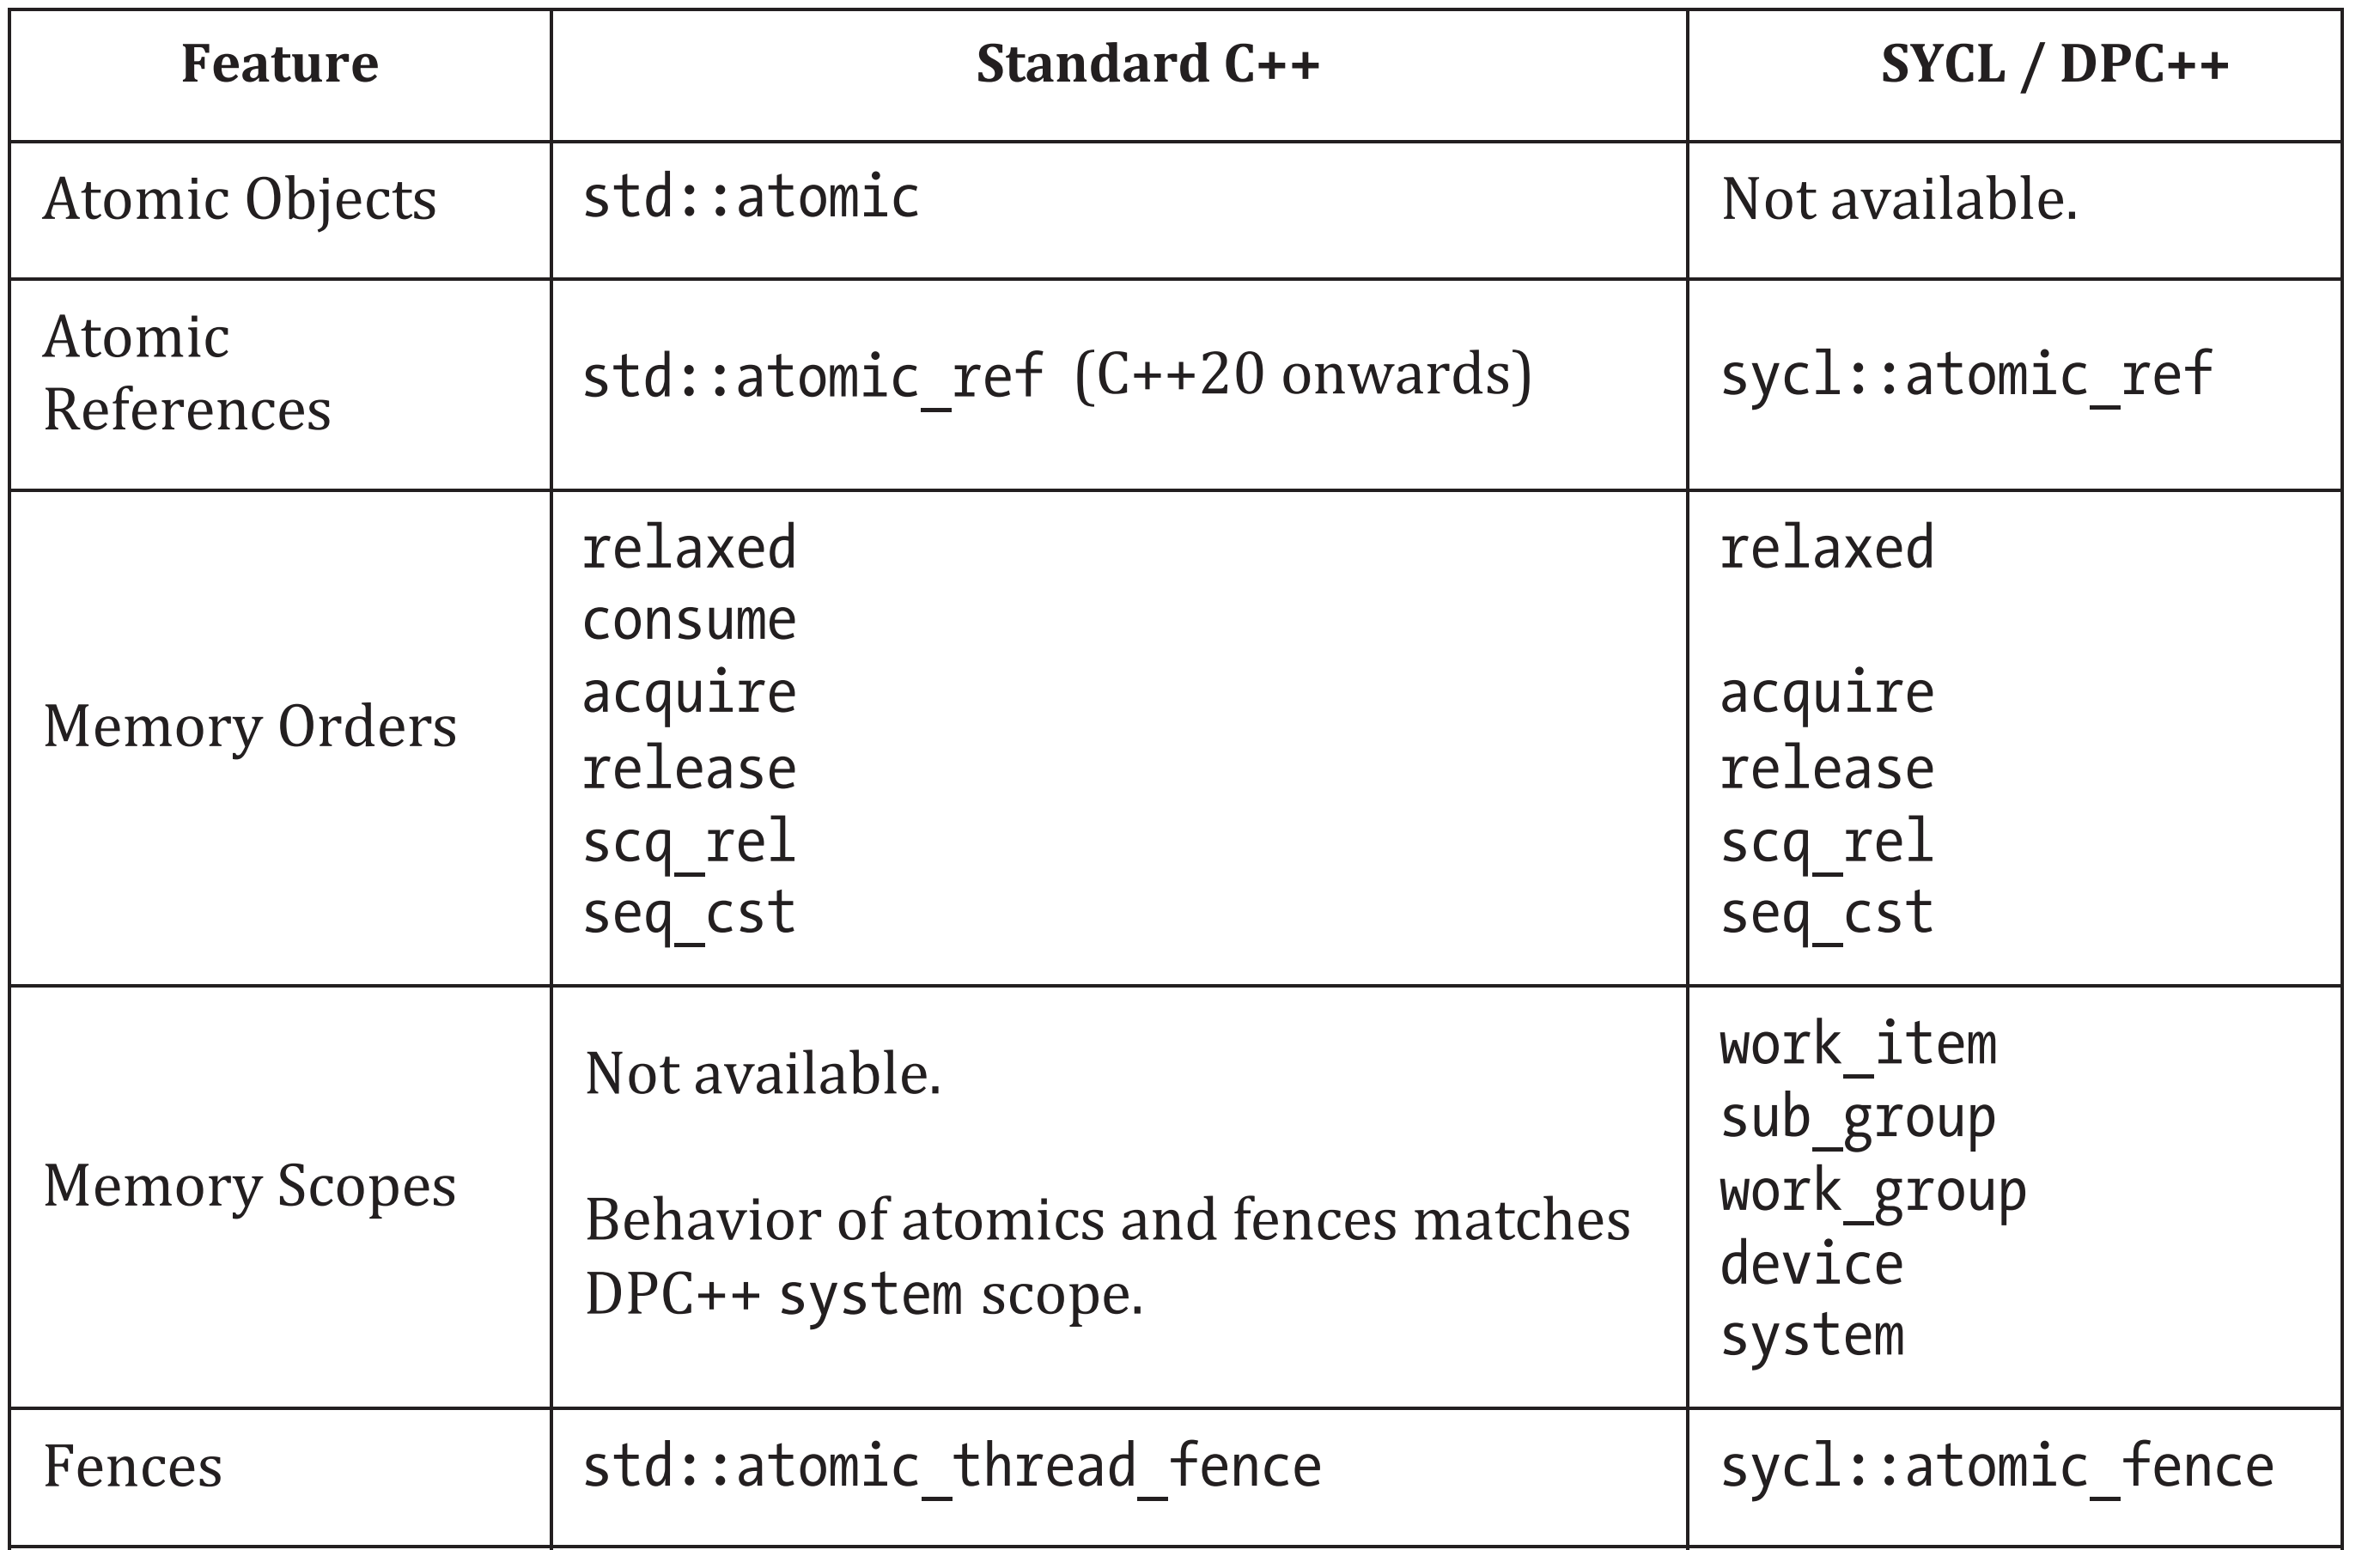
\includegraphics[width=1.0\textwidth]{content/chapter-19/images/6}
	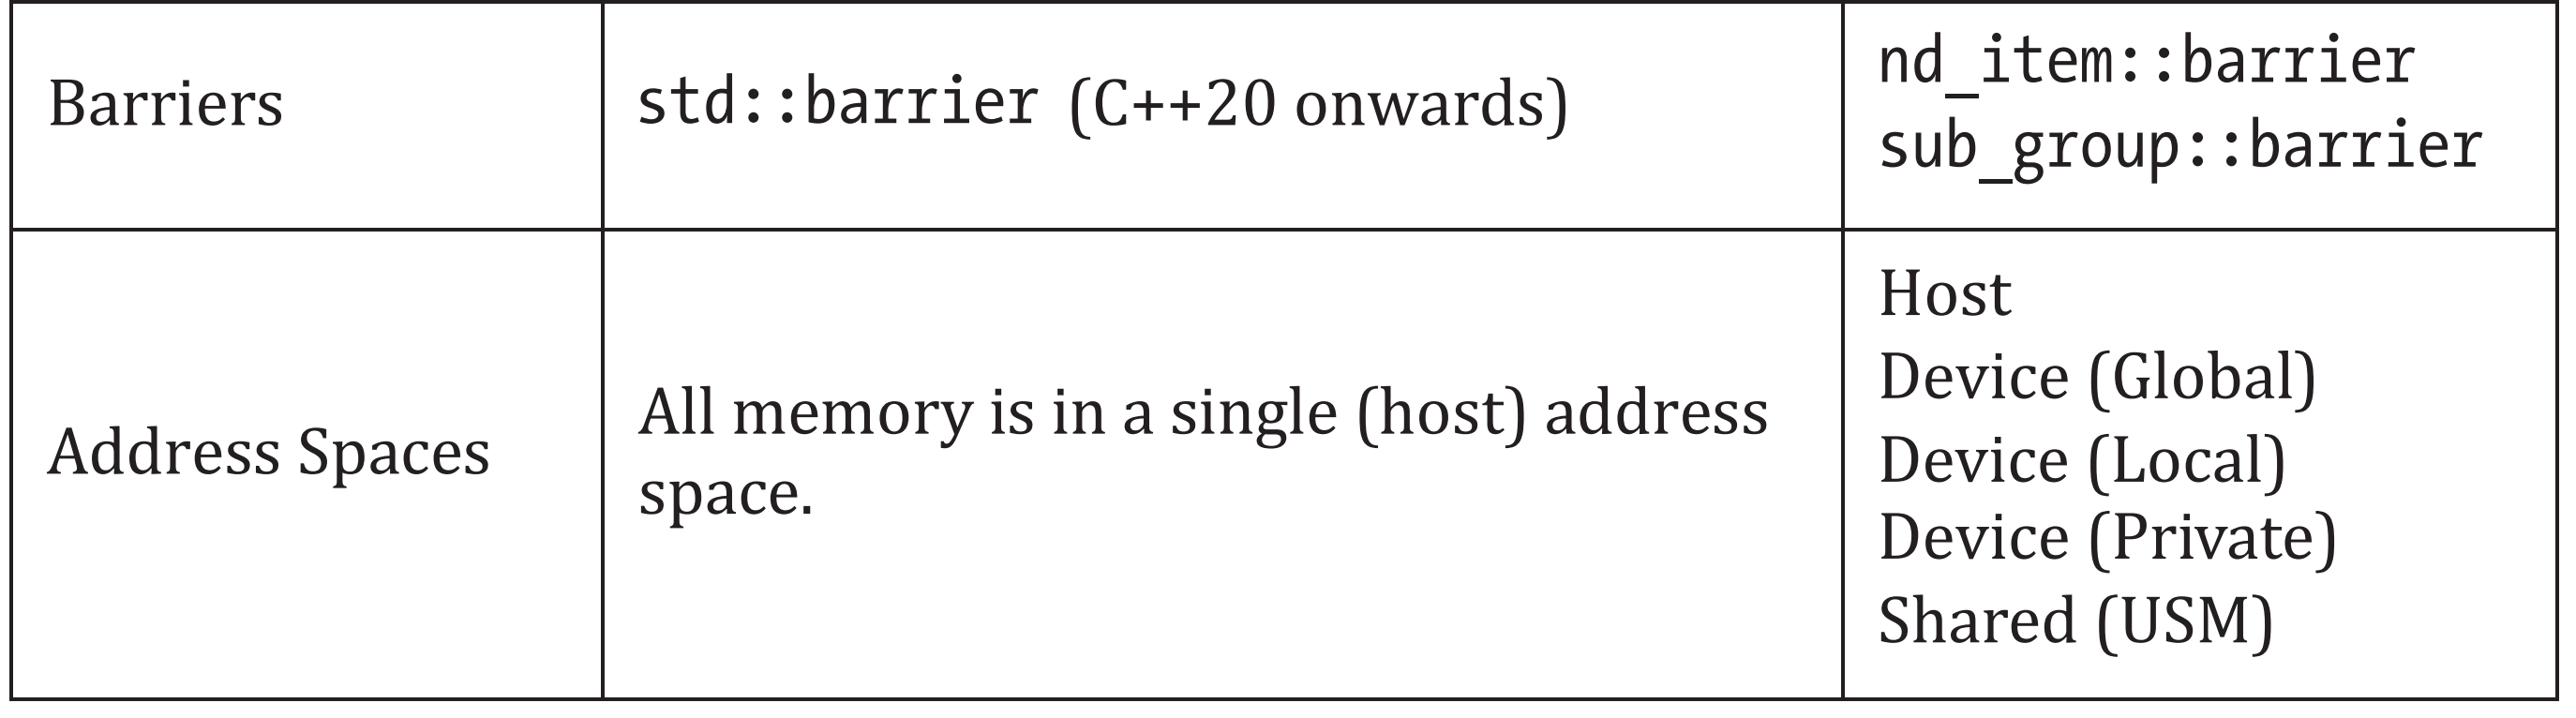
\includegraphics[width=1.0\textwidth]{content/chapter-19/images/7}
\end{center}

\hspace*{\fill} \par %插入空行
\textbf{The memory\_order Enumeration Class}

The memory model exposes different memory orders through six values of the memory\_order enumeration class, which can be supplied as arguments to fences and atomic operations. Supplying a memory order argument to an operation tells the compiler what memory ordering guarantees are required for all other memory operations (to any address) relative to that operation, as explained in the following:\par

\begin{itemize}
	\item memory\_order::relaxed \\
	Read and write operations can be re-ordered before or after the operation with no restrictions. There are no ordering guarantees.
	\item memory\_order::acquire \\
	Read and write operations appearing after the operation in the program must occur after it (i.e., they cannot be re-ordered before the operation).
	\item memory\_order::release \\ 
	Read and write operations appearing before the operation in the program must occur before it (i.e., they cannot be re-ordered after the operation), and preceding write operations are guaranteed to be visible to other program instances which have been synchronized by a corresponding acquire operation (i.e., an atomic operation using the same variable and memory\_order::acquire or a barrier function).
	\item memory\_order::acq\_rel \\
	The operation acts as both an acquire and a release. Read and write operations cannot be re-ordered around the operation, and preceding writes must be made visible as previously described for memory\_order::release.
	\item memory\_order::seq\_cst \\
	The operation acts as an acquire, release, or both depending on whether it is a read, write, or read-modify-write operation, respectively. All operations with this memory order are observed in a sequentially consistent order.
\end{itemize}

There are several restrictions on which memory orders are supported by each operation. The table in Figure 19-10 summarizes which combinations are valid.\par

\hspace*{\fill} \par %插入空行
Figure 19-10. Supporting atomic operations with memory\_order
\begin{center}
	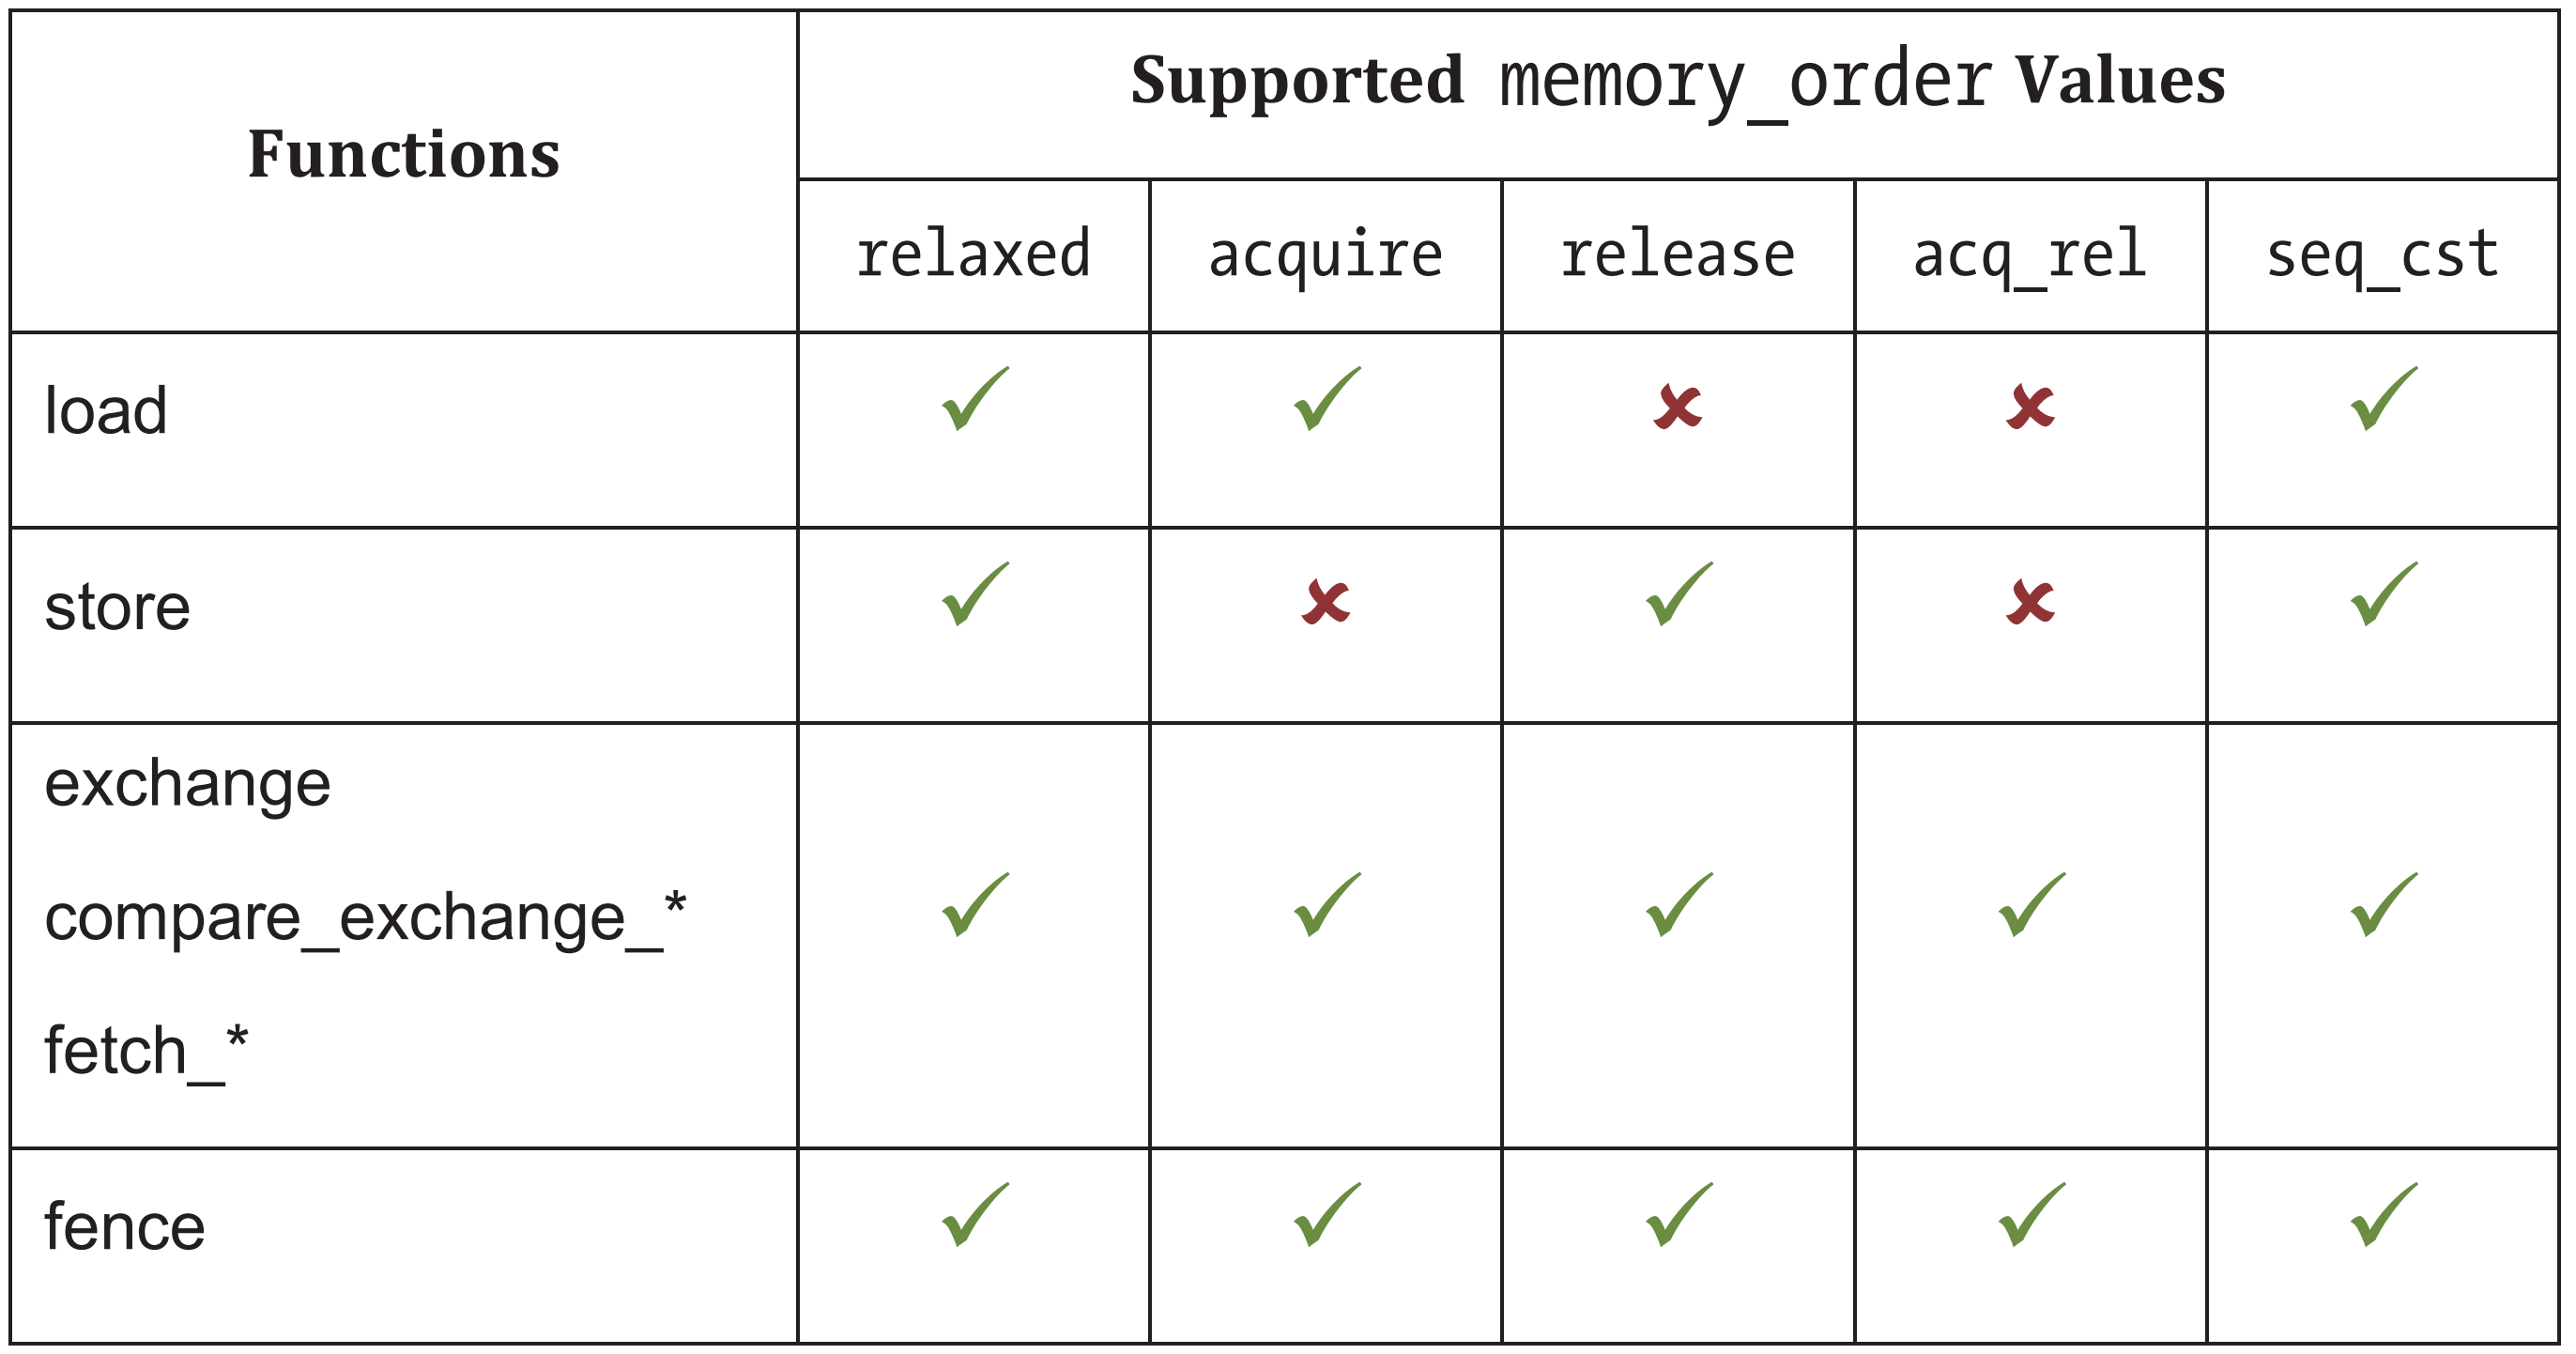
\includegraphics[width=1.0\textwidth]{content/chapter-19/images/8}
\end{center}

Load operations do not write values to memory and are therefore incompatible with release semantics. Similarly, store operations do not read values from memory and are therefore incompatible with acquire semantics. The remaining read-modify-write atomic operations and fences are compatible with all memory orderings.\par

\begin{tcolorbox}[colback=blue!5!white,colframe=blue!75!black, title=MEMORY ORDER IN C++]
The C++ memory model additionally includes memory\_order::consume, with similar behavior to memory\_order::acquire. However, the C++17 standard discourages its use, noting that its definition is being revised. Its inclusion in DPC++ has therefore been postponed to a future version.
\end{tcolorbox}

\hspace*{\fill} \par %插入空行
\textbf{The memory\_scope Enumeration Class}

The standard C++ memory model assumes that applications execute on a single device with a single address space. Neither of these assumptions holds for DPC++ applications: different parts of the application execute on different devices (i.e., a host device and one or more accelerator devices); each device has multiple address spaces (i.e., private, local, and global); and the global address space of each device may or may not be disjoint (depending on USM support).\par

In order to address this, DPC++ extends the C++ notion of memory order to include the scope of an atomic operation, denoting the minimum set of work-items to which a given memory ordering constraint applies. The set of scopes are defined by way of a memory\_scope enumeration class:\par

\begin{itemize}
	\item memory\_scope::work\_item \\
	The memory ordering constraint applies only to the calling work-item. This scope is only useful for image operations, as all other operations within a work-item are already guaranteed to execute in program order.
	\item memory\_scope::sub\_group, memory\_scope::work\_
	group \\
	The memory ordering constraint applies only to work-items in the same sub-group or work-group as the calling work-item.
	\item memory\_scope::device \\ 
	The memory ordering constraint applies only to work-items executing on the same device as the calling work-item.
	\item memory\_scope::system \\
	The memory ordering constraint applies to all workitems in the system.
\end{itemize}

Barring restrictions imposed by the capabilities of a device, all memory scopes are valid arguments to all atomic and fence operations. However, a scope argument may be automatically demoted to a narrower scope in one of three situations:\par

\begin{enumerate}
	\item If an atomic operation updates a value in workgroup local memory, any scope broader than 	memory\_scope::work\_group is narrowed (because local memory is only visible to work-items in the same work-group).
	\item If a device does not support USM, specifying memory\_scope::system is always equivalent to memory\_scope::device (because buffers cannot be accessed concurrently by multiple devices).
	\item If an atomic operation uses memory\_order::relaxed, there are no ordering guarantees, and the memory scope argument is effectively ignored.
\end{enumerate}

\hspace*{\fill} \par %插入空行
\textbf{Querying Device Capabilities}

To ensure compatibility with devices supported by previous versions of SYCL and to maximize portability, DPC++ supports OpenCL 1.2 devices and other hardware that may not be capable of supporting the full C++ memory model (e.g., certain classes of embedded devices). DPC++ provides device queries to help us reason about the memory order(s) and memory scope(s) supported by the devices available in a system:\par

\begin{itemize}
	\item atomic\_memory\_order\_capabilities \\
	atomic\_fence\_order\_capabilities \\
	Return a list of all memory orderings supported by atomic and fence operations on a specific device. All devices are required to support at least memory\_order::relaxed, and the host device is required to support all memory orderings.
	\item atomic\_memory\_scope\_capabilities \\
	atomic\_fence\_scope\_capabilities \\
	Return a list of all memory scopes supported by atomic and fence operations on a specific device. All devices are required to support at least memory\_order::work\_group, and the host device is required to support all memory scopes.
\end{itemize}

It may be difficult at first to remember which memory orders and scopes are supported for which combinations of function and device capability. In practice, we can avoid much of this complexity by following one of the two development approaches outlined in the following:\par

\begin{enumerate}
	\item Develop applications with sequential consistency and system fences.\\
	Only consider adopting less strict memory orders during performance tuning.
	\item Develop applications with relaxed consistency and work-group fences. \\
	Only consider adopting more strict memory orders and broader memory scopes where required for correctness.
\end{enumerate}

The first approach ensures that the semantics of all atomic operations and fences match the default behavior of standard C++. This is the simplest and least error-prone option, but has the worst performance and portability characteristics.\par

The second approach is more aligned with the default behavior of previous versions of SYCL and languages like OpenCL. Although more complicated—since it requires that we become more familiar with the different memory orders and scopes—it ensures that the majority of the DPC++ code we write will work on any device without performance penalties.\par

\hspace*{\fill} \par %插入空行
\textbf{Barriers and Fences}

All previous usages of barriers and fences in the book so far have ignored the issue of memory order and scope, by relying on default behavior.\par

Every group barrier in DPC++ acts as an acquire-release fence to all address spaces accessible by the calling work-item and makes preceding writes visible to at least all other work-items in the same group. This ensures memory consistency within a group of work-items after a barrier, in line with our intuition of what it means to synchronize (and the definition of the synchronizes-with relation in C++).\par

The atomic\_fence function gives us more fine-grained control than this, allowing work-items to execute fences with a specified memory order and scope. Group barriers in future versions of DPC++ may similarly accept an optional argument to adjust the memory scope of the acquirerelease fences associated with a barrier\par

\hspace*{\fill} \par %插入空行
\textbf{Atomic Operations in DPC++}

DPC++ provides support for many kinds of atomic operations on a variety of data types. All devices are guaranteed to support atomic versions of common operations (e.g., loads, stores, arithmetic operators), as well as the atomic compare-and-swap operations required to implement lock-free algorithms. The language defines these operations for all fundamental integer, floating-point, and pointer types—all devices must support these operations for 32-bit types, but 64-bit-type support is optional.\par

\hspace*{\fill} \par %插入空行
\textbf{The atomic Class}

The std::atomic class from C++11 provides an interface for creating and operating on atomic variables. Instances of the atomic class own their data, cannot be moved or copied, and can only be updated using atomic operations. These restrictions significantly reduce the chances of using the class incorrectly and introducing undefined behavior. Unfortunately, they also prevent the class from being used in DPC++ kernels—it is impossible to create atomic objects on the host and transfer them to the device! We are free to continue using std::atomic in our host code, but attempting to use it inside of device kernels will result in a compiler error.\par

\begin{tcolorbox}[colback=blue!5!white,colframe=blue!75!black, title=ATOMIC CLASS DEPRECATED IN SYCL 2020 AND DPC++]
The SYCL 1.2.1 specification included a cl::sycl::atomic class that is loosely based on the std::atomic class from C++11. We say loosely because there are some differences between the interfaces of the two classes, most notably that the SYCL 1.2.1 version does not own its data and defaults to a relaxed memory ordering.\\

The cl::sycl::atomic class is fully supported by DPC++, but its use is discouraged to avoid confusion. We recommend that the atomic\_ref class (covered in the next section) be used in its place.
\end{tcolorbox}

\hspace*{\fill} \par %插入空行
\textbf{The atomic\_ref Class}

The std::atomic\_ref class from C++20 provides an alternative interface for atomic operations which provides greater flexibility than std::atomic. The biggest difference between the two classes is that instances of std::atomic\_ref do not own their data but are instead constructed from an existing non-atomic variable. Creating an atomic reference effectively acts as a promise that the referenced variable will only be accessed atomically for the lifetime of the reference. These are exactly the semantics needed by DPC++, since they allow us to create non-atomic data on the host, transfer that data to the device, and treat it as atomic data only after it has been transferred. The atomic\_ref class used in DPC++ kernels is therefore based on std::atomic\_ref.\par

We say based on because the DPC++ version of the class includes three additional template arguments as shown in Figure 19-11.\par

\hspace*{\fill} \par %插入空行
Figure 19-11. Constructors and static members of the atomic\_ref class
\begin{lstlisting}[caption={}]
template <typename T,
			memory_order DefaultOrder,
			memory_scope DefaultScope, 
			access::address_space AddressSpace>
class atomic_ref {
public:
	using value_type = T;
	static constexpr size_t required_alignment =
		/* implementation-defined */;
	static constexpr bool is_always_lock_free =
		/* implementation-defined */;
	static constexpr memory_order default_read_order =
		memory_order_traits<DefaultOrder>::read_order;
	static constexpr memory_order default_write_order =
		memory_order_traits<DefaultOrder>::write_order;
	static constexpr memory_order default_read_modify_write_order =
		DefaultOrder;
	static constexpr memory_scope default_scope = DefaultScope;
	
	explicit atomic_ref(T& obj);
	atomic_ref(const atomic_ref& ref) noexcept;
};
\end{lstlisting}

As discussed previously, the capabilities of different DPC++ devices are varied. Selecting a default behavior for the atomic classes of DPC++ is a difficult proposition: defaulting to standard C++ behavior (i.e., memory\_order::seq\_cst, memory\_scope::system) limits code to executing only on the most capable of devices; on the other hand, breaking with C++ conventions and defaulting to the lowest common denominator (i.e., memory\_order::relaxed, memory\_scope::work\_group) could lead to unexpected behavior when migrating existing C++ code. The design adopted by DPC++ offers a compromise, allowing us to define our desired default behavior as part of an object’s type (using the DefaultOrder and DefaultScope template arguments). Other orderings and scopes can be provided as runtime arguments to specific atomic operations as we see fit—the DefaultOrder and DefaultScope only impact operations where we do not or cannot override the default behavior (e.g., when using a shorthand operator like +=). The final template argument denotes the address space in which the referenced object is allocated.\par

An atomic reference provides support for different operations depending on the type of object that it references. The basic operations supported by all types are shown in Figure 19-12, providing the ability to atomically move data to and from memory.\par

\hspace*{\fill} \par %插入空行
Figure 19-12. Basic operations with atomic\_ref for all types
\begin{lstlisting}[caption={}]
void store(T operand,
	memory_order order = default_write_order,
	memory_scope scope = default_scope) const noexcept;
T operator=(T desired) const noexcept; // equivalent to store

T load(memory_order order = default_read_order,
	memory_scope scope = default_scope) const noexcept;
operator T() const noexcept; // equivalent to load

T exchange(T operand,
	memory_order order = default_read_modify_write_order,
	memory_scope scope = default_scope) const noexcept;
	
bool compare_exchange_weak(T &expected, T desired,
	memory_order success,
	memory_order failure,
	memory_scope scope = default_scope) const noexcept;
	
bool compare_exchange_weak(T &expected, T desired,
	memory_order order = default_read_modify_write_order,
	memory_scope scope = default_scope) const noexcept;
	
bool compare_exchange_strong(T &expected, T desired,
	memory_order success,
	memory_order failure,
	memory_scope scope = default_scope) const noexcept;
	
bool compare_exchange_strong(T &expected, T desired,
	memory_order order = default_read_modify_write_order,
	memory_scope scope = default_scope) const noexcept;
\end{lstlisting}

Atomic references to objects of integral and floating-point types extend the set of available atomic operations to include arithmetic operations, as shown in Figures 19-13 and 19-14. Devices are required to support atomic floating-point types irrespective of whether they feature native support for floating-point atomics in hardware, and many devices are expected to emulate atomic floating-point addition using an atomic compare exchange. This emulation is an important part of providing performance and portability in DPC++, and we should feel free to use floating-point atomics anywhere that an algorithm requires them—the resulting code will work correctly everywhere and will benefit from future improvements in floating-point atomic hardware without any modification!\par

\hspace*{\fill} \par %插入空行
Figure 19-13. Additional operations with atomic\_ref only for integral types
\begin{lstlisting}[caption={}]
Integral fetch_add(Integral operand,
	memory_order order = default_read_modify_write_order,
	memory_scope scope = default_scope) const noexcept;
	
Integral fetch_sub(Integral operand,
	memory_order order = default_read_modify_write_order,
	memory_scope scope = default_scope) const noexcept;
	
Integral fetch_and(Integral operand,
	memory_order order = default_read_modify_write_order,
	memory_scope scope = default_scope) const noexcept;
	
Integral fetch_or(Integral operand,
	memory_order order = default_read_modify_write_order,
	memory_scope scope = default_scope) const noexcept;
	
Integral fetch_min(Integral operand,
	memory_order order = default_read_modify_write_order,
	memory_scope scope = default_scope) const noexcept;

Integral fetch_max(Integral operand,
	memory_order order = default_read_modify_write_order,
	memory_scope scope = default_scope) const noexcept;

Integral operator++(int) const noexcept;
Integral operator--(int) const noexcept;
Integral operator++() const noexcept;
Integral operator--() const noexcept;
Integral operator+=(Integral) const noexcept;
Integral operator-=(Integral) const noexcept;
Integral operator&=(Integral) const noexcept;
Integral operator|=(Integral) const noexcept;
Integral operator^=(Integral) const noexcept;
\end{lstlisting}

\hspace*{\fill} \par %插入空行
Figure 19-14. Additional operations with atomic\_ref only for floating-point types
\begin{lstlisting}[caption={}]
Floating fetch_add(Floating operand,
	memory_order order = default_read_modify_write_order,
	memory_scope scope = default_scope) const noexcept;
	
Floating fetch_sub(Floating operand,
	memory_order order = default_read_modify_write_order,
	memory_scope scope = default_scope) const noexcept;
	
Floating fetch_min(Floating operand,
	memory_order order = default_read_modify_write_order,
	memory_scope scope = default_scope) const noexcept;
	
Floating fetch_max(Floating operand,
	memory_order order = default_read_modify_write_order,
	memory_scope scope = default_scope) const noexcept;
	
Floating operator+=(Floating) const noexcept;
Floating operator-=(Floating) const noexcept;
\end{lstlisting}

\hspace*{\fill} \par %插入空行
\textbf{Using Atomics with Buffers}

As discussed in the previous section, there is no way in DPC++ to allocate atomic data and move it between the host and device. To use atomic operations in conjunction with buffers, we must create a buffer of nonatomic data to be transferred to the device and then access that data through an atomic reference.\par

\hspace*{\fill} \par %插入空行
Figure 19-15. Accessing a buffer via an explicitly created atomic\_ref
\begin{lstlisting}[caption={}]
Q.submit([&](handler& h) {
	accessor acc{buf, h};
	h.parallel_for(N, [=](id<1> i) {
		int j = i % M;
		atomic_ref<int, memory_order::relaxed, memory_scope::system,
				access::address_space::global_space> atomic_acc(acc[j]);
		atomic_acc += 1;
	});
});
\end{lstlisting}

The code in Figure 19-15 is an example of expressing atomicity in DPC++ using an explicitly created atomic reference object. The buffer stores normal integers, and we require an accessor with both read and write permissions. We can then create an instance of atomic\_ref for each data access, using the += operator as a shorthand alternative for the fetch\_add member function.\par

This pattern is useful if we want to mix atomic and non-atomic accesses to a buffer within the same kernel, to avoid paying the performance overheads of atomic operations when they are not required. If we know that only a subset of the memory locations in the buffer will be accessed concurrently by multiple work-items, we only need to use atomic references when accessing that subset. Or, if we know that work-items in the same work-group only concurrently access local memory during one stage of a kernel (i.e., between two work-group barriers), we only need to use atomic references during that stage.\par

Sometimes we are happy to pay the overhead of atomicity for every access, either because every access must be atomic for correctness or because we’re more interested in productivity than performance. For such cases, DPC++ provides a shorthand for declaring that an accessor must always use atomic operations, as shown in Figure 19-16.\par

\hspace*{\fill} \par %插入空行
Figure 19-16. Accessing a buffer via an atomic\_ref implicitly created by an atomic accessor
\begin{lstlisting}[caption={}]
buffer buf(data);

Q.submit([&](handler& h) {
	atomic_accessor acc(buf, h, relaxed_order, system_scope);
	h.parallel_for(N, [=](id<1> i) {
		int j = i % M;
		acc[j] += 1;
	});
});
\end{lstlisting}

The buffer stores normal integers as before, but we replace the regular accessor with a special atomic\_accessor type. Using such an atomic accessor automatically wraps each member of the buffer using an atomic reference, thereby simplifying the kernel code.\par

Whether it is best to use the atomic reference class directly or via an accessor depends on our use case. Our recommendation is to start with the accessor for simplicity during prototyping and initial development, only moving to the more explicit syntax if necessary during performance tuning (i.e., if profiling reveals atomic operations to be a performance bottleneck) or if atomicity is known to be required only during a well-defined phase of a kernel (e.g., as in the histogram code later in the chapter).\par

\hspace*{\fill} \par %插入空行
\textbf{Using Atomics with Unified Shared Memory}

As shown in Figure 19-17 (reproduced from Figure 19-7), we can construct atomic references from data stored in USM in exactly the same way as we could for buffers. Indeed, the only difference between this code and the code shown in Figure 19-15 is that the USM code does not require buffers or accessors.\par

\hspace*{\fill} \par %插入空行
Figure 19-17. Accessing a USM allocation via an explicitly created atomic\_ref
\begin{lstlisting}[caption={}]
q.parallel_for(range<1>(N), [=](size_t i) {
	int j = i % M;
	atomic_ref<int, memory_order::relaxed, memory_scope::system,
				access::address_space::global_space> atomic_data(data[j]);
	atomic_data += 1;
}).wait();
\end{lstlisting}

There is no way of using only standard DPC++ features to mimic the shorthand syntax provided by atomic accessors for USM pointers. However, we expect that a future version of DPC++ will provide a shorthand built on top of the mdspan class that has been proposed for C++23.\par























